\section{STL简介}
\textbf{标准模板库(Standard template library, STL)}主要借助C++的泛型编程来完成,但它又在泛型编程之外引入了许多新的概念,比如迭代器(Iterator)和函数对象(Function object/Functor)。本节仅对STL中的容器(Container)、迭代器、函数对象和算法(Algorithm)作简单介绍;至于更深入、更复杂的内容,就让我们留到精讲篇吧。\par
STL的内容十分博杂,本书无法尽述。读者若是想要使用某个STL工具,最好提前查阅相关文档,了解其具体使用方式及其注意事项,比如:
\begin{itemize}
    \item \href{https://zh.cppreference.com/w/cpp/container}{STL容器库 - cppreference.com}
    \item \href{https://zh.cppreference.com/w/cpp/iterator}{STL迭代器库 - cppreference.com}
    \item \href{https://zh.cppreference.com/w/cpp/utility/functional}{STL函数对象 - cppreference.com}
    \item \href{https://zh.cppreference.com/w/cpp/algorithm}{STL算法库 - cppreference.com}
\end{itemize}
\subsection*{STL容器}
容器,顾名思义,就是用来容纳某种事物的。比如说 \lstinline@std::vector@,它可以改变长度,同时像数组那样容纳 \lstinline@T@ 类型的数据;而 \lstinline@std::forward_list@ 是单链表,它可以像我们第六章中写的单链表那样,链式存储 \lstinline@T@ 类型的数据(当然,也可以改变长度)。\par
\subsubsection*{顺序容器}
我们已经对部分STL容器(如 \lstinline@std::vector@ 和 \lstinline@std::array@)相当熟悉了。它们都属于顺序容器(Sequence Container)。\textbf{顺序容器的特点是,一个容器内所存的所有单元(元素)在逻辑上是按照确定的先后次序排布的——或者说,线性排布的\footnote{注意:逻辑上的先后次序不代表内存中的排布次序,比如单链表/双链表,它们在内存中的分布没有任何规律,但它们在逻辑上具有确定的先后次序。}。}\par
\lstinline@std::forward_list@ 是单链表容器,它的每一个单元都只包含向后(next)\footnote{数据结构中的``向前''和``向后''表示的含义是模糊的,一般要取决于语境。有些时候我们称下一个元素为``前一个'',而有些时候我们却下一个元素为``后一个''。这可能是翻译或者其它方面的不统一导致的,因为英文语境中的``previous''和``next''是表意明确的。}的指针,而没有向前(previous)的指针;\lstinline@std::list@ 是双链表,它的每一个单元都包含向前和向后的指针,所以我们可以任意地进行向前和向后查找——代价就是,每个元素要用额外的内存空间来存储向前的指针值。\par
\lstinline@std::deque@ 表示一个双端队列,它允许我们在容器的首尾快速插入/删除元素。虽然 \lstinline@std::vector@ 也能在末尾快速插入/删除元素,但是它操作头部元素插入/删除的效率就很低(第一位以后的数据将会依次后移,然后待处理数据才能插入第一位)。
\begin{lstlisting}
#include <deque>
#include <string>
int main() {
    std::deque<std::string> dogs {"Husky", "Samoyed", "Alaskan"};
    dogs.push_front("Retriever"); //std::deque插入首元素效率更高
    dogs.pop_front(); //删除首元素同理
\end{lstlisting}\par
总而言之,各种顺序容器都有各自的优缺点,我们可以根据自己在实际编程中的需要,选择使用不同的容器。\par
\subsubsection*{关联容器}
顺序容器可以方便我们根据下标(索引值)快速访问对应的内容值(\lstinline@std::array@, \lstinline@std::vector@ 及 \lstinline@std::deque@),或者为插入/删除特定数据提供方便(\lstinline@std::forward_list@ 及 \lstinline@std::list@)。而\textbf{关联容器(Associative container)可以通过元素排序,为我们快速查找信息提供便利。}我们来着重讲一下这部分内容。\par
\lstinline@std::set@ 表示一个集合。对于一个 \lstinline@std::set@ 的对象来说,每个元素就是一个\textbf{键(Key)}。如果键的类型 \lstinline@Key@ 重载了 \lstinline@<@ 运算符,那么 \lstinline@std::set<Key>@ 就可以正常使用;否则编译器会报错。\par
\begin{lstlisting}
#include <set>
#include <string>
int main() {
    std::set<std::string> mathematicians { //键的类型为std::string
        "Euclid", "Pythagoras", "Archimedes", "Newton"
    }, physicists {
        "Galileo", "Kepler", "Newton"
    };
    if (mathematicians.find("Newton") != mathematicians.end())
        std::cout << "Newton is a mathematician.\n"; //在某集合中查找某个键
    physicists.insert("Einstein"); //向某集合中插入某个键
    if (physicists.erase("Euclid")) //尝试从physicists中移除"Euclid"
        std::cout << "Euclid is removed from physicists.\n"; 
\end{lstlisting}
这段代码的运行结果如下:\\\noindent\rule{\linewidth}{.2pt}\texttt{
Newton is a mathematician.
}\\\noindent\rule{\linewidth}{.2pt}\par
\lstinline@std::set@ 有一个特点,它不允许键重复。如果一个集合中已经存在某个键,那么插入相同的值将没有任何作用(什么也不做)。因此,我们可以利用 \lstinline@std::set@ 的这种元素不重复特性来进行数据去重(稍后我们会看到一个这样的例子)。\par
\lstinline@find@ 成员函数用于在集合中寻找一个键;如果找到了,返回对应位置的迭代器;如果没找到,返回 \lstinline@end()@ 成员迭代器。所以我们只需要判断它是否等于 \lstinline@end()@ 成员,就能知道这个集合中有没有我们想要找的那个键了。
\begin{lstlisting}
    if (mathematicians.find("Newton") != mathematicians.end()) { /*...*/ }
\end{lstlisting}\par
\lstinline@insert@ 成员函数用于在集合中插入一个键。如果这个键早已存在,那么 \lstinline@insert@ 将什么也不做,以此保证键不重复。
\begin{lstlisting}
    physicists.insert("Einstein"); //向某集合中插入某个键
    physicists.insert("Einstein"); //"Einstein"已经存在,本次插入将什么也不做
\end{lstlisting}
\lstinline@insert@ 成员函数还有大量的重载,但是本节只是简介,就不细讲了。\par
\lstinline@erase@ 成员函数可以从集合中删除一个键,并返回一个 \lstinline@std::size_t@ 结果,表示删除了多少个键——对于不允许元素重复的 \lstinline@std::set@ 来说当然只能有 \lstinline@0@ 或 \lstinline@1@ 两种可能。如果该集合中本来就没有这个键,那么 \lstinline@erase@ 就什么也不做,并返回 \lstinline@0@。
\begin{lstlisting}
    if (physicists.erase("Euclid")) { /*...*/ };
\end{lstlisting}\par
读者或许会发现,\lstinline@std::set@ 的很多成员函数名与 \lstinline@std::string@, \lstinline@std::vector@ 都很相似。这是STL容器\footnote{包括不属于STL但在很多方面与其十分相似的伪容器 \lstinline@std::string@。}的一大特点:执行相似功能的函数有相似的名字\footnote{还记得我们说过的 \lstinline@std::string::size()@ 吗?它和 \lstinline@std::string::length()@ 完全等价,但它是为了模仿STL容器而设的成员函数。}和参数类型。这样的好处是既方便我们记忆和使用不同容器的同类功能,又方便我们对容器类型进行进一步抽象(我们会在讲算法时看到这一点)。\par
接下来我们写一段简单的代码,借助 \lstinline@std::set@ 的功能,来删除 \lstinline@std::list@ 中的重复元素。
\lstinputlisting[caption=\texttt{remove\_duplicate.cpp}]{code_in_book/11.7/remove_duplicate.cpp}
这段代码的运行结果是:\\\noindent\rule{\linewidth}{.2pt}\texttt{
c a b d e
}\\\noindent\rule{\linewidth}{.2pt}
可以看到,这个运行结果实现了去重的效果,很好地符合了我们的预期\footnote{顺便一说,算法库中的 \lstinline@std::unique@ 和容器自带的 \lstinline@std::list::unique@ 函数都能实现一定程度上的去重效果,但它们并不是我们想要的那种去重;或者说,我们需要先排序元素,再去重。}。此外,这里涉及了一点迭代器的使用,这是因为 \lstinline@std::list::erase@ 只支持迭代器作为实参。稍后我们就会讲解迭代器。\par
\lstinline@map@ 也是一个关联容器,它表示的是映射\footnote{在数学上,映射可以描述为两组值的对应关系。对于每个$x\in\mathbb A$,依照某种映射规则$f$,总有唯一确定的$y\in\mathbb B$与之对应,那么我们称$f$为一个从$\mathbb A$到$\mathbb B$的映射。}。这个类模板有两个(无默认值的)模板参数,一个是键类型 \lstinline@Key@,一个是值类型 \lstinline@T@。我们可以用 \lstinline@insert@ 成员函数向 \lstinline@std::map@ 对象中添加\textbf{键-值对(Key-value pair)},这之后我们就可以通过键来找到相应的值。
\begin{lstlisting}
#include <map>
int main() {
    std::map<std::string, int> birth_year{
        {"Bjarne Stroustrup", 1950}, //一个键-值对
        {"Donald Knuth", 1938},
        {"Linus Torvalds", 1969},
        {"Alan Turing", 1912}
    }; //建立一个birth_year映射
    birth_year.insert(std::make_pair("Tim Berners-Lee", 1955));
    //std::map的插入操作比较特殊,读者可以自行查阅相关资料
    std::cout << birth_year["Bjarne Stroustrup"]; //输出1950
    //可以用下标运算符,通过键找到对应的值
\end{lstlisting}
\lstinline@std::map@ 允许我们通过下标运算符来接收键,并输出对应的值。这样一来,我们也就不必局限于数组那种只能接收整型数据的下标了——只要你愿意,你可以使用任何类型(只要它重载有 \lstinline@<@ 运算符)作为下标!\par
\lstinline@std::multiset@ 和 \lstinline@std::multimap@ 与 \lstinline@std::set@ 和 \lstinline@std::map@ 相差不大,只是前两者允许键重复,而后两者不允许键重复而已。不过,\lstinline@std::multimap@ 不再重载下标运算符,这是因为键不唯一,我们不能单纯根据一个键的信息来锁定唯一一个值。\par
\subsubsection*{无序关联容器}
\textbf{无序关联容器(Unordered associative container)}是以上四个关联容器的无序版本,包括 \lstinline@std::unordered_set@, \lstinline@std::unordered_map@, \lstinline@std::unordered_multiset@ 及 \lstinline@std::unordered_multimap@。\par
无序关联容器不使用 \lstinline@<@ 运算符来排序,而是通过 \lstinline@std::hash@ 建立散列表\footnote{散列(Hash)是一种压缩数据的方法,它可以根据一定的算法,把任何一种数据压缩成一个整数,或者一段字符串,从而方便检索等操作。散列处理过程不可避免地造成信息,所以散列计算是不可逆的,这也使得它在数据保护方面大有用武之地。}来存储信息。我们就不展开讲了。\par
相较而言,无序关联容器的数据检索效率比有序关联容器更高;但它也有更大的内存空间占用。在实际操作中,我们可以根据自己的实际需要来选择使用有序关联容器还是无序关联容器。\par
\subsubsection*{容器适配器}
\textbf{容器适配器(Container adapter)}是对STL已有容器进行适当的功能改造而得到的容器。截至C++17,STL库一共为我们提供了三种容器适配器:\lstinline@std::stack@, \lstinline@std::queue@ 和 \lstinline@std::priority_queue@。\par
\lstinline@std::stack@ 表示一个栈(Stack)结构(线性),即只能从末尾插入或删除元素,而不能在其它位置插入或删除元素的容器。我们之前也曾用私有继承的方式完成过一个简单的 \lstinline@stack@。\par
\lstinline@std::queue@ 表示一个队列(Queue)结构(线性),即只能从末尾插入元素和从头部删除元素的容器。我们不能从队列的末尾删除元素或者从头部插入元素,也不能在中间插入/删除元素。这个容器可以通过适配 \lstinline@std::deque@ 来获得,读者可以自行尝试。\par
\lstinline@std::priority_queue@ 表示一个堆(Heap)结构(非线性)\footnote{即便如此,它也还是针对顺序容器适配得到的,只是它表示了非线性的结构而已。}。当我们插入一个值时,堆会以这个值的大小(这个类型需要支持 \lstinline@<@)排序,并把更大的值排在顶端。当弹出元素时,堆会优先把顶端元素——也就是最大的数据弹出。所以,如果我们需要进行数据排序的话,\lstinline@std::multiset@ 和 \lstinline@std::priority_queue@ 都是不错的选择;\lstinline@std::set@ 一般来说不是,因为它会把相同的数据丢掉,这往往不合我们的需要。
\begin{lstlisting}
#include <queue> //priority_queue定义于queue库中
int main() {
    int arr[] {2,6,3,8,1,3,2,7,3,4,9};
    std::priority_queue<int> pq;
    for (auto x : arr)
        pq.push(x); //把arr的每个元素都移入堆中
    while (pq.size()) {
        std::cout << pq.top() << ' '; //输出顶端元素
        pq.pop(); //弹出顶端元素
    } //将输出9 8 7 6 4 3 3 3 2 2 1
\end{lstlisting}\par
\subsection*{迭代器}
迭代器是STL中最具特色的概念,它是指针概念的推广。为了解释清楚迭代器存在的意义,我们就来想这样一个问题吧:试想,对于一个 \lstinline@std::vector<int>@ 来说,如果我希望用一个指针指向它的某个数据——比如第一个元素,那么我们只需要一个 \lstinline@int*@ 指针就可以完成这个操作。
\begin{lstlisting}
    std::vector<int> vec {1,2,3,4,5};
    int *pvec {&vec[0]}; //vec[0]返回的是对vec首元素的引用
\end{lstlisting}
这样就解决了,很简单吧。\par
那么对玗一个 \lstinline@std::list<int>@ 来说,我们也可以用 \lstinline@int*@ 指针指向它的第一个元素。只不过 \lstinline@std::list@ 没有对下标运算符的重载,我们需要使用 \lstinline@front()@ 成员函数。
\begin{lstlisting}
    std::list<int> lst {1,2,3,4,5};
    int *plst {&lst.front()}; //front()返回的是对lst首元素的引用
\end{lstlisting}
这样也可以解决。\par
那么我们为什么要使用``指针''呢?如果要修改某个元素的内容,我们直接用这个容器/这个容器的引用不好吗?\par
首先,有些可以用指针来表达的东西并不是``容器'',比如说原始的数组,我们可以用指针来表达它,但是我们不能把它当作一个容器,它既不是类模板,也没有成员函数。假如我们要写一个算法,它的参数可以是任何一种线性数据结构,那么我们就必须在各种顺序容器/容器适配器之外为数组单独设计一个重载——还是接收指针参数版本的。所以,如果我们能设计一个只需要指针参数的函数,把各种容器的元素也都用指针表示,那该多方便啊。\par
其次,虽然STL的容器对于相同操作一般使用同样的函数名,但是它们还是在某些地方有些细微差别的。比如,同样是在末尾插入元素,\lstinline@std::vector@ 和 \lstinline@std::list@ 的函数名为 \lstinline@push_back@;而 \lstinline@std::stack@ 和 \lstinline@std::queue@ 的函数名则是 \lstinline@pop@(因为只能从末尾插入元素)。同样是在头部移除元素,\lstinline@std::deque@ 的函数名是 \lstinline@pop_front@,而 \lstinline@std::queue@ 的函数名是 \lstinline@pop@(因为只能从头部移除元素)。如果考虑到这些差别,那么我们还需要再为不同的容器写不同的代码,这就一下子把问题又变复杂了。\par
然而,``指针''这个思路虽然好,但它也有自己的问题。举个例子吧,请问如何表示 \lstinline@pvec@ 所指元素的``下一个''元素的地址?读者可能很快就想到了,当然是 \lstinline@pvec+1@ 啊,因为在内存中,\lstinline@std::vector@ 的元素就是连续排布的。那么如何表示 \lstinline@plst@ 所指元素的``下一个''元素的地址?读者可能也会下意识地想到 \lstinline@plst+1@,但这是错的!只要回顾一个第六章中我们讲过的内容,读者就会明白,链表中的元素在内存中并不连续排布,所以 \lstinline@plst+1@ 得不到我们想要的结果。同样的道理,\lstinline@std::deque@ 的元素在内存中是分块排布的\footnote{详见 \href{https://stackoverflow.com/a/6292437/22112284}{What really is a deque in STL? - Stack Overflow} 的回答。},我们对指针 \lstinline@+1@ 也不一定能得到想要的结果。\par
\begin{figure}[htbp]
    \centering
    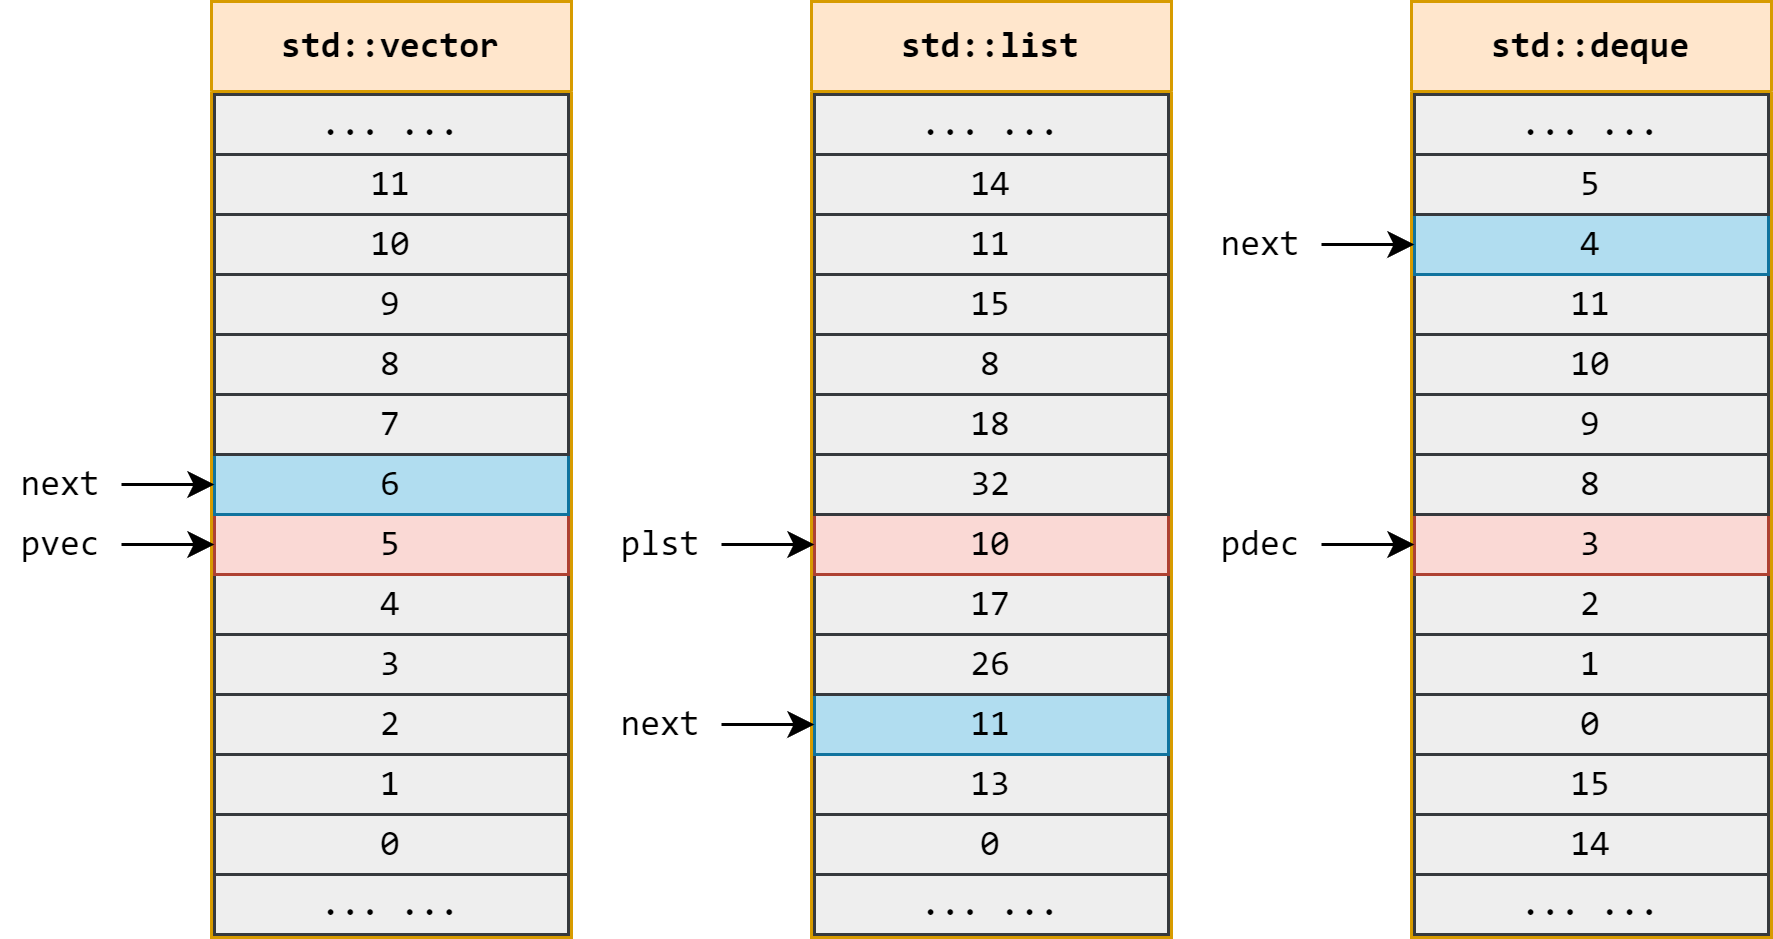
\includegraphics[width=\textwidth]{../images/generalized_parts/11_different_types_of_pointer_to_containers.png}
    \caption{使用裸指针的问题——谁是``下一个''元素?}
\end{figure}
不同的容器有各自的实现方式,这就使我们使用指针的想法很难实现。在这种情况下,``迭代器''的概念就应运而生了,它在表现上如同平凡的指针,但是在求``下一个元素''的时候,却能有方便又统一的方法。\par
每个容器都有内置的迭代器类型。比如 \lstinline@std::list@ 的迭代器类型就叫 \lstinline@std::list<T,Allocator>::iterator@。这个类重载了 \lstinline@++@ 运算符,使得它的对象在自增时,不是像指针那样在地址值上加一个 \lstinline@sizeof(T)@,而是根据 \lstinline@std::list@ 的特点,把这个对象的指向变成``下一个元素''\footnote{至于具体如何实现,不同容器自有不同办法,我们不必深究。}。\par
迭代器有不同的种类,能支持的功能也存在一定区别。对于 \lstinline@std::list@ 所具备的双向迭代器(我们稍后简述)来说,它有如下特征:
\begin{itemize}
    \item 重载了 \lstinline@*@ 运算符,使我们可以读写某个元素的内容(很像指针吧)。
    \item 重载了 \lstinline@++@ 和 \lstinline@--@ 运算符,包括前缀和后缀版本,使我们可以向前或向后移动迭代器的指向(很像指针,只不过它不是单纯在地址上作自增/自减了)。
    \item 虽然它很像指针,但是我们不能在 \lstinline@T*@ 类型与迭代器类型之间进行类型转换。
\end{itemize}\par
\lstinline@std::list@ 有成员函数 \lstinline@begin()@,它的返回值就是指向首个元素的迭代器;还有成员函数 \lstinline@end()@,它的返回值是指向末尾元素的``下一个元素''的迭代器。换句话说,\lstinline@begin()@ 和 \lstinline@end()@ 可以构成一组左闭右开的迭代器序列$[$ \lstinline@begin(), end()@ $)$,在此区间之内的是有效信息。\footnote{初学者可能对此感到十分困惑,但这样设计自有它的好处。比如说,当一段范围为空时,\lstinline@begin()@ 就与 \lstinline@end()@ 相等,这就很方便我们进行判断;一段范围有多长,可以直接根据 \lstinline@begin()@ 自增到与 \lstinline@end()@ 相等的次数来得出。}\par
\begin{figure}[htbp]
    \centering
    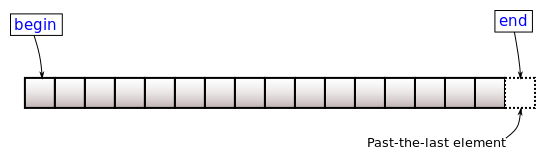
\includegraphics[width=.8\textwidth]{../images/generalized_parts/11_range_begin_end.png}
    \caption{\lstinline@begin()@ 到 \lstinline@end()@ 的范围}
    \footnotesize{图片来源:cppreference}
\end{figure}
接下来这段代码是通过迭代器实现的简单遍历操作,我们在 \lstinline@for@ 循环内按顺序输出 \lstinline@std::list<int>@ 的数据。\par
\begin{lstlisting}
    std::list<int> lst {1,2,3,4,5};
    for (
        std::list<int>::iterator it = lst.begin(); //it指向lst的首元素
        it != lst.end(); //如果it还没到lst的末尾,就继续循环
        it++ //it++就能使它指向下一个元素
    )
        std::cout << *it << ' '; //可以用取内容运算符访问it指向的内容
\end{lstlisting}\par
这个 \lstinline@for@ 循环是从 \lstinline@lst.begin()@ 开始的。关于这个首元素,我们还有另一种写法:\lstinline@std::begin(lst)@。\lstinline@std::begin()@ 是非成员函数,它的效果与 \lstinline@lst.begin()@ 相同,不过它可以支持那些没有 \lstinline@begin()@ 成员函数的类型,没错,就是数组。
\begin{lstlisting}
    int arr[3] {1,2,3};
    for (int *pi = std::begin(arr); pi != std::end(arr); pi++) { /*...*/ }
\end{lstlisting}\par
回来看前一段代码。这里的 \lstinline@it@ 是一个迭代器类型,它是 \lstinline@std::list<int>@ 的公有内嵌类。如果我你嫌这种写法太麻烦,没关系,我们可以用 \lstinline@auto@,交给编译器来推导类型。
\begin{lstlisting}
    for (auto it = std::begin(lst); it != std::end(lst); it++) { /*...*/ }
    //编译器会根据std::begin(lst)的类型,推导出it的类型
\end{lstlisting}
这个循环的条件是 \lstinline@it!=std::end(lst)@,也就是说,\lstinline@it@ 在自增的过程中还没有走到 \lstinline@end@ 处。如果它走到了 \lstinline@end@,那就该结束循环了,因为 \lstinline@end@ 不指向有效信息。\par
还记得我们曾讲过的范围 \lstinline@for@ 循环吗?其实它也是基于迭代器的。我们可以把上述代码简化成这样,效果相同:
\begin{lstlisting}
    for (auto it : lst) { /*...*/ }
\end{lstlisting}
迭代器是STL中的一种重要的工具,大多数算法库中的算法都要依赖于它;许多容器的成员函数也会用到它。当然,我们也可以在自己写的 \lstinline@user::array@ 容器中添加迭代器。我们留待精讲篇介绍。\par
\subsubsection*{迭代器的一种分类}
不同容器有不同迭代器类,这些迭代器实现的功能可以存在差异。比如说,\lstinline@std::array<T,N>::iterator@ 支持下标运算符和加减法,就像真的指针一样。这当然是因为 \lstinline@std::array@ 本身是用数组实现的,而数组支持这些类似指针的加减和下标运算。\par
但 \lstinline@std::list<T>::iterator@ 就不行了,这当然也是因为它是用链表实现的,在读取元素时只能一步一步往前探(自增),或者一步一步往后退(自减),不能一下子跳好多个元素。\par
\lstinline@std::forward_list<T>::iterator@ 不仅不支持下标和加减法,还不能支持自减运算,只能自增。这是因为单链表的每个元素没有指向上一个元素的指针,只能指向下一个元素,因而它的迭代器也只能朝着单个方向走,不能回头。\par
你看,不同的迭代器在行为上可能有不少差别,所以我们需要依据迭代器能够执行的操作进行分类。
\begin{itemize}
    \item 输出迭代器(Output iterator)可以支持程序向容器或输出设备中写入(输出)内容,支持自增操作。
    \item 输入迭代器(Input iterator)可以支持程序从容器或输入设备中读取(输入)内容,支持自增操作。
    \item 前向迭代器(Forward iterator)具有输入迭代器的特点\footnote{我们可以认为,前向迭代器是一种特殊的输入迭代器。},同时还必须支持有多趟的自增操作\footnote{有多趟的自增操作意味着这种迭代器在能够自增的前提下还需要满足一些条件,详见 \href{https://zh.cppreference.com/w/cpp/named_req/ForwardIterator\#.E5.A4.9A.E8.B6.9F.E4.BF.9D.E8.AF.81}{C++具名要求:老式向前迭代器\#多趟保证 - cppreference.com}}。有些迭代器还应支持输出操作,即同时具有输出迭代器和输入迭代器的特点\footnote{笔者认为,这未尝不是一种多重继承。}。
    \item 双向迭代器(Bidirectional iterator)具有前向迭代器的特点,同时还支持自减操作,即向后移动。\lstinline@std::list@ 的迭代器属于这类。
    \item 随机访问迭代器(Random access iterator)具有双向迭代器的特点,同时还支持加减运算、下标、比较运算符等随机访问\footnote{
        随机访问(Random Access)是指能够在常量时间内访问数据结构中的任意元素的能力,比如数组的下标访问;与之相对的是“顺序访问”(Sequential Access),在顺序访问中,访问元素的时间取决于元素在数据结构中的位置。}特性。\lstinline@std::deque@ 的迭代器属于这类。另外,裸指针也可以视为一种随机访问迭代器。
    \item 连续迭代器(Contiguous iterator)具有随机访问迭代器的特点,同时必须要求这个容器的内容是连续存储的。\lstinline@std::vector@ 和 \lstinline@std::array@ 的迭代器属于这类。
\end{itemize}
我们可以列一个有关它们功能支持情况的简表,见表11.1。限于篇幅,这里就不再详细阐述了,我把它们放到精讲篇。
\begin{table}[htbp]
\centering
\begin{tabular}{cccccccc}
\hline\rule{0pt}{2.4ex}
\multirow{3}{*}{迭代器类型} & \multicolumn{7}{c}{操作和存储要求}\\
\cline{2-8}\rule{0pt}{2.4ex}
& \multirow{2}{*}{输出} & \multirow{2}{*}{输入} & \multicolumn{2}{c}{自增} & \multirow{2}{*}{有多趟自减} & \multirow{2}{*}{随机访问} & \multirow{2}{*}{连续存储}\\
\cline{4-5}\rule{0pt}{2.4ex}
& & & 无多趟 & 有多趟 & & &\\
\hline\hline\rule{0pt}{2.4ex}
输出迭代器 & 支持 & & 支持\\
\hline\rule{0pt}{2.4ex}
输入迭代器 & & 支持 & 支持\\
\hline\rule{0pt}{2.4ex}
前向迭代器 & 可能支持 & 支持 & 支持 & 支持\\
\hline\rule{0pt}{2.4ex}
双向迭代器 & 可能支持 & 支持 & 支持 & 支持 & 支持\\
\hline\rule{0pt}{2.4ex}
随机访问迭代器 & 可能支持 & 支持 & 支持 & 支持 & 支持 & 支持\\
\hline\rule{0pt}{2.4ex}
连续迭代器 & 可能支持 & 支持 & 支持 & 支持 & 支持 & 支持 & 支持\\
\hline
\end{tabular}
\caption{迭代器类型,及其支持的特性}
\footnotesize{留空表示``不需要支持''}
\end{table}
\subsection*{函数对象}
函数对象与函数指针、闭包之间的关系比较密切;但是泛讲篇中都没有讲到,所以我们也不会把函数对象讲得太深。\par
我们根据接收参数的个数(一般不超过两个),把STL中的函数对象所代表的函数分成三类:
\begin{itemize}
    \item 生成器(Generator)不接收任何参数,它只负责产生一个值。对于比较简单的情形来说,因为它不接收参数,所以只要外界条件不变,这种函数总会返回相同的值\footnote{因为全局变量等的存在,事实并非总是如此。不过读者暂且这样理解就好}。这些函数可以返回值,也可以有副作用,下同。
    \item 一元函数(Unary function)只接收一个参数。如果某个一元函数的返回类型是 \lstinline@bool@,那么我们把它称为谓词(Predicate)\footnote{``谓词''这个名字有它的道理,但是很容易让初学者觉得莫名其妙——就像``对象''这个名字,不知有多少初学者在此处犯过迷糊。这些高大上的名字实在是不接地气,不便于学习。}。
    \item 二元函数(Binary function)接收两个参数。如果某个二元函数的返回类型是 \lstinline@bool@,那么我们把它称为二元谓词(Binary predicate)。
\end{itemize}
这些概念非并必须掌握的,但是理解它们并加以区分,会对我们设计算法有大有裨益。\par
函数是函数,对象是对象,它们本应该是泾渭分明的,彼此没有任何关系;但是有些对象却可以被当作``函数''来调用。听上去是不是玄之又玄?还是让我们来看一个例子吧:\lstinline@functional@ 库中定义有 \lstinline@plus@ 类模板,它的声明是:
\begin{lstlisting}
template< class T = void >
struct plus;
\end{lstlisting}
至于成员,它只有一个重载函数调用运算符 \lstinline@()@ 是我们需要的,除此之外就是一些我们用不上的 \lstinline@using@ 语句。
\begin{lstlisting}
//简化的定义
template <class _Ty = void>
struct plus {
    using _FIRST_ARGUMENT_TYPE_NAME _CXX17_DEPRECATE_ADAPTOR_TYPEDEFS  = _Ty;
    using _SECOND_ARGUMENT_TYPE_NAME _CXX17_DEPRECATE_ADAPTOR_TYPEDEFS = _Ty;
    using _RESULT_TYPE_NAME _CXX17_DEPRECATE_ADAPTOR_TYPEDEFS          = _Ty;
    //上面这些不用管,我们用不上
    constexpr _Ty operator()(const _Ty &_Left, const _Ty &_Right)const {
        return _Left + _Right;
    } //重载函数调用运算符
};
\end{lstlisting}
这个成员函数的返回值是 \lstinline@_Ty@,即与参数一样的类型。而它的定义,只不过是把两个参数加起来而已,看上去没什么玄乎的。重载函数调用运算符也没什么可怕的,其实和重载下标运算符的使用方式很像,只是参数个数不一定是单个了。
\begin{lstlisting}
    std::plus<int> intplus;
    std::cout << intplus.operator()(1, 2) << '\n'; //完整写法
    std::cout << intplus(1, 2) << '\n'; //一般写法
\end{lstlisting}
对于那个完整写法来说,\lstinline@operator()@ 就是成员函数名;而后面套的括号就是参数列表。我们还可以简化一下,写成下一行中的一般写法。你发现了吗?这种写法和函数调用一模一样。如果没有上下文的话,我们可能真的会把 \lstinline@intplus@ 当成一个函数。这就是重载函数调用运算符 \lstinline@()@ 的效果。\par
其实 \lstinline@std::integral_constant@ 也有重载函数调用运算符。因此我们也可以把 \lstinline@std::is_same@ 的对象当作函数来调用\footnote{别忘了,\lstinline@std::is_same@ 继承自 \lstinline@std::integral_constant<bool,v>@,所以它也继承了这个函数调用运算符。}。
\begin{lstlisting}
    std::cout << std::is_same<int[], int[3]>{}();
\end{lstlisting}
我们来分析下这段代码。首先,\lstinline@std::is_same<int[],int[3]>@ 它本身是一个类,而不是对象,所以它是没办法调用非静态成员的\footnote{顺便一说,函数调用运算符不能定义为静态成员函数。}。所以我们要先用花括号构造一个临时的函数对象,接下来再调用这个成员函数,那么一切就顺理成章了。\par
读者可能会想:``你说的这个 \lstinline@std::is_same@ 例子使用函数调用运算符确实有点用处,能简化代码;但是我为什么要用那个 \lstinline@std::plus@?我直接用加法运算符还不行吗?\lstinline@std::plus<int>{}(1,2)@ 和 \lstinline@1+2@ 哪个更方便?''
其实,这些函数对象的存在,不是为了简化计算,而是出于另一种目的——传参。试想,我们可以把一个对象作为参数传递给某个函数,但我们要怎么把一个运算符传递给某个函数?而 \lstinline@functional@ 库中的这些函数类模板\footnote{它们又叫运算符包装器(Operator wrapper)。}则能产生相应的对象,然后传递给对应的函数,使``传入一个运算符''成为可能。\par
\subsection*{算法}
STL的算法库十分精彩,包含我们在日常编程中经常使用的各种功能,比如排序、搜索、批处理、数值运算等。我们来看几个例子;如果算法本身很简单,我们也可以直接实现出来。\par
算法库中的大部分是函数模板,它们往往要依赖迭代器与函数对象。下面我们来介绍一个只依赖迭代器就可以完成的 \lstinline@std::copy@ 函数,它定义于 \lstinline@algorithm@ 库中。
\begin{lstlisting}
template<class InputIt, class OutputIt>
OutputIt copy(InputIt first, InputIt last, OutputIt d_first);
\end{lstlisting}
这个算法的含义是,把从 \lstinline@first@ 到 \lstinline@last@ 位置(左包含,右不包含,下同)的内容拷贝到 \lstinline@d_first@ 起的若干位置。至于返回值,就是待复制区域的``下一个''位置。\par
\begin{figure}[htbp]
    \centering
    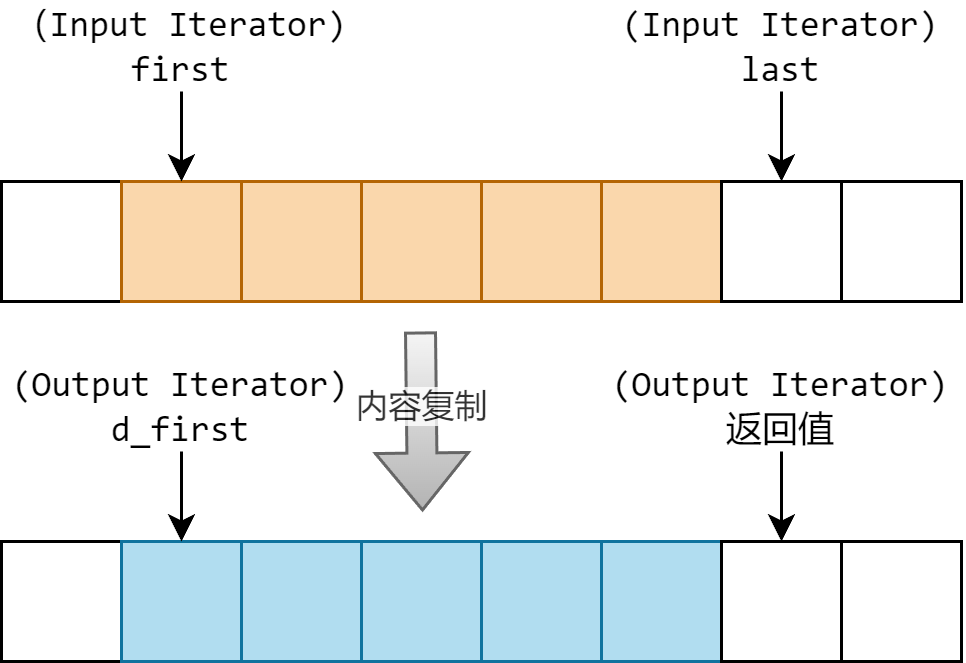
\includegraphics[width=.6\textwidth]{../images/generalized_parts/11_algorithm_copy.png}
    \caption{\lstinline@copy@ 算法的含义}
\end{figure}
读者会发现,在这里我们已经不考虑容器的类型了。不管它是数组,还是 \lstinline@std::vector@,还是 \lstinline@std::deque@ 或者 \lstinline@std::list@,乃至非顺序容器 \lstinline@std::set@ 及 \lstinline@std::map@,反正它们都至少满足前向迭代器的要求,那么对于输入/输出迭代器来说自然是不在话下。所以算法是与容器类型无关的,它只需要考虑迭代器的类型;至于迭代器类型如何,那才是容器说了算的——这是一种对容器类型的抽象。\par
这个算法很容易实现,我们自己都可以写一份出来。
\begin{lstlisting}
//namespace user
template<typename InputIt, typename OutputIt>
OutputIt copy(
    InputIt first,
    InputIt last,
    OutputIt d_first
) {
    for (; 
        first != last; //如果first不等于last,就说明还有未拷贝的值
        ++first, ++d_first //分别对两个迭代器自增,它们都会指向“下一个”元素
    )
        *d_first = *first; //彼值赋为此值,又完成了一个元素的拷贝
    return d_first; //返回值刚好就是待复制区域的“下一个”位置
}
\end{lstlisting}
这里的 \lstinline@for@ 循环迭代语句部分执行了两个操作,是用逗号隔开的,表示的意思就是同时相加。除此之外没有什么要讲了,这个操作本身很简单。\par
\lstinline@std::sort@ 和 \lstinline@std::stable_sort@ 是两种排序算法。它们都可以对 \lstinline@first@ 到 \lstinline@last@ 之间的内容进行排序。
\begin{lstlisting}
template<class RandomIt>
void sort(RandomIt first, RandomIt last); //(1)
template<class RandomIt, class Compare>
void sort(RandomIt first, RandomIt last, Compare comp); //(2)
template<class RandomIt>
void stable_sort(RandomIt first, RandomIt last); //(3)
template<class RandomIt, class Compare>
void stable_sort(RandomIt first, RandomIt last, Compare comp); //(4)
\end{lstlisting}
其中(2)(4)的 \lstinline@comp@ 参数代表二元谓词,含义为比较。对于(1)(3)来说,它们默认使用小于号作为谓词。如果使用小于号作为谓词,那么排序出来的结果将是从小到大的:
\begin{lstlisting}
    int arr[5] {4,3,2,5,1};
    std::sort(arr, arr + 5); //从小到大排序
    for (auto x : arr)
        std::cout << x << ' '; //输出1 2 3 4 5
\end{lstlisting}
我们可以传入一个二元谓词函数对象,以此改变它们的排序方案,比如说大于号对应的函数对象 \lstinline@std::greater@。
\begin{lstlisting}
    std::sort(arr, arr + 5, std::greater<int>{}); //从大到小排序
    for (auto x : arr)
        std::cout << x << ' '; //输出5 4 3 2 1
\end{lstlisting}\par
\lstinline@std::stable_sort@ 与 \lstinline@std::sort@ 的区别在于,前者不会改变相等元素的顺序,而后者不在乎相等元素的顺序。对于基本数据类型的内容来说,相等元素之间的顺序确实无所谓;但是对于自定义类型来说,那可就不一定了。
\begin{lstlisting}
struct Student {
    unsigned ID; //唯一的编号
    unsigned score; //成绩
    bool operator<(const Student &stu)const { //以供根据成绩排序
        return score < stu.score;
    }
};
\end{lstlisting}
这是一个很简单的例子,但足够明确。对于 \lstinline@Student@ 类来说,两个对象``相等''只是意味着它们的 \lstinline@score@ 成员相等,但不判断编号的值。因此,``相等''并不意味着两个对象的所有成员完全相同!否则我们就该说``考了相同分数的就是同一个人'',这太荒谬了。\par
所以回到 \lstinline@std::stable_sort@,这个算法不会改变相等元素的顺序,其实就是保证了分数相同的学生仍然按照它们原来的相互顺序来排序,而不致顺序错乱。\lstinline@std::sort@ 就不管这个了。\par
\lstinline@std::for_each@ 是一种批处理算法。
\begin{lstlisting}
template<class InputIt, class UnaryFunction>
UnaryFunction for_each(InputIt first, InputIt last, UnaryFunction f);
\end{lstlisting}
它的含义是,对 \lstinline@first@ 到 \lstinline@last@ 之间的每个数都进行 \lstinline@f@ 操作。鉴于 \lstinline@functional@ 库中没有表示自增/自减的运算符包装器,我们就自己写一个。很简单,我们只要写一个函数调用运算符重载就行了。
\begin{lstlisting}
//namespace user
template<typename T>
struct increment { //表示前缀自增
    T& operator()(T &value)const{ //const仅表明increment对象可以是常量
        ++value;
        return value;
    }
};
\end{lstlisting}
接下来我们就可以利用这个前缀自增运算符的对象,通过 \lstinline@for_each@来进行批处理了。
\begin{lstlisting}
    std::deque<int> deq {4,3,2,5,1};
    std::for_each(deq.begin(), deq.end(), user::increment<int>{});
    for (auto x : deq)
        std::cout << x << ' '; //输出5 4 3 6 2
\end{lstlisting}\par
这个算法的实现也很简单,我们可以试着来写一下:
\begin{lstlisting}
//namespace user
template<typename InputIt, typename UnaryFunction>
UnaryFunction for_each(
    InputIt first,
    InputIt last,
    UnaryFunction f
) {
    for (; first != last; ++first)
        f(*first);
    return f;
}
\end{lstlisting}
其实它就是对 \lstinline@first@ 到 \lstinline@last@ 之间所指的每一个对象进行 \lstinline@f@ 处理嘛,没什么难的。\par
不过读者可能会好奇,这里我们直接改变形参 \lstinline@first@ 的指向,不会影响实参 \lstinline@deq.begin()@ 的指向吗?当然不会,因为我们传参时传递的是迭代器对象,而不是迭代器引用。所以形参 \lstinline@first@ 也只是一个临时变量,和实参 \lstinline@deq.begin()@ 的地址是不同的,它们互不影响。
如果读者不适应这种写法的话,那么我们再定义一个中介迭代器 \lstinline@it@ 参与循环也未为不可。
\begin{lstlisting}
    for (InputIt it = first; it != last; ++it) //效果相同
        f(*it);
\end{lstlisting}\par
\lstinline@std::lexicographical_compare@ 也是一个算法。
\begin{lstlisting}
template<class InputIt1, class InputIt2>
bool lexicographical_compare(InputIt1 first1, InputIt1 last1,
                             InputIt2 first2, InputIt2 last2);
template<class InputIt1, class InputIt2, class Compare>
bool lexicographical_compare(InputIt1 first1, InputIt1 last1,
                             InputIt2 first2, InputIt2 last2, Compare comp);
\end{lstlisting}
它的含义是,按照小于号或者 \lstinline@comp@ 谓词,对 \lstinline@first1@ 到 \lstinline@last1@ 和 \lstinline@first2@ 到 \lstinline@last2@ 的部分进行字典序比较。它的实现说难不也难,说易也不易,我就陈列其中一个在这里,感兴趣的读者可以自己瞧瞧。
\begin{lstlisting}
//namespace user
template<class InputIt1, class InputIt2, class Compare>
bool lexicographical_compare(
    InputIt1 first1, InputIt1 last1, //Input1和Input2可以不同
    InputIt2 first2, InputIt2 last2, //意味着允许跨容器类型进行比较
    Compare comp
) {
    for (; (first1 != last1) && (first2 != last2); ++first1, ++first2)
        if (comp(*first1, *first2))
            return true;
        else if (comp(*first2, *first1))
            return false;
    return (first1 == last1) && (first2 != last2);
}
\end{lstlisting}\par
